
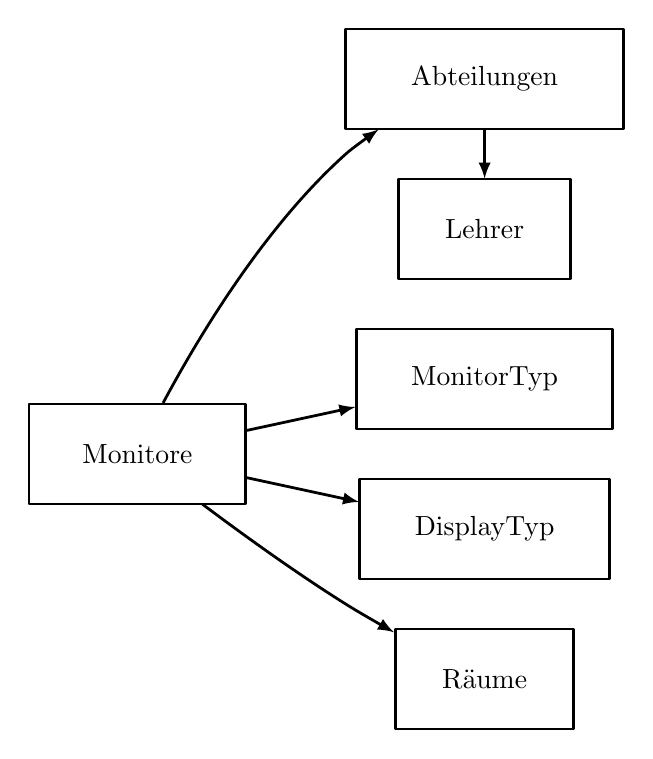
\begin{tikzpicture}[>=latex,line join=bevel,]
  \pgfsetlinewidth{1bp}
%%
\pgfsetcolor{black}
  % Edge: Abteilungen -> Lehrer
  \draw [->] (164bp,215.79bp) .. controls (164bp,213.31bp) and (164bp,210.83bp)  .. (164bp,198.14bp);
  % Edge: Monitore -> MonitorTyp
  \draw [->] (78.208bp,107.47bp) .. controls (87.551bp,109.49bp) and (97.705bp,111.68bp)  .. (117.49bp,115.95bp);
  % Edge: Monitore -> Räume
  \draw [->] (62.441bp,80.929bp) .. controls (76.965bp,70.036bp) and (96.187bp,56.157bp)  .. (114bp,45bp) .. controls (116.76bp,43.272bp) and (119.64bp,41.541bp)  .. (131.38bp,34.83bp);
  % Edge: Monitore -> Abteilungen
  \draw [->] (48.255bp,117.4bp) .. controls (60.657bp,140.61bp) and (84.558bp,180.68bp)  .. (114bp,207bp) .. controls (115.13bp,208.01bp) and (116.3bp,208.99bp)  .. (125.86bp,215.91bp);
  % Edge: Monitore -> DisplayTyp
  \draw [->] (78.208bp,90.531bp) .. controls (87.974bp,88.422bp) and (98.626bp,86.121bp)  .. (118.82bp,81.759bp);
  % Node: Lehrer
\begin{scope}
  \definecolor{strokecol}{rgb}{0.0,0.0,0.0};
  \pgfsetstrokecolor{strokecol}
  \draw (195bp,198bp) -- (133bp,198bp) -- (133bp,162bp) -- (195bp,162bp) -- cycle;
  \draw (164bp,180bp) node {Lehrer};
\end{scope}
  % Node: Räume
\begin{scope}
  \definecolor{strokecol}{rgb}{0.0,0.0,0.0};
  \pgfsetstrokecolor{strokecol}
  \draw (196bp,36bp) -- (132bp,36bp) -- (132bp,0bp) -- (196bp,0bp) -- cycle;
  \draw (164bp,18bp) node {Räume};
\end{scope}
  % Node: Monitore
\begin{scope}
  \definecolor{strokecol}{rgb}{0.0,0.0,0.0};
  \pgfsetstrokecolor{strokecol}
  \draw (78bp,117bp) -- (0bp,117bp) -- (0bp,81bp) -- (78bp,81bp) -- cycle;
  \draw (39bp,99bp) node {Monitore};
\end{scope}
  % Node: Abteilungen
\begin{scope}
  \definecolor{strokecol}{rgb}{0.0,0.0,0.0};
  \pgfsetstrokecolor{strokecol}
  \draw (214bp,252bp) -- (114bp,252bp) -- (114bp,216bp) -- (214bp,216bp) -- cycle;
  \draw (164bp,234bp) node {Abteilungen};
\end{scope}
  % Node: MonitorTyp
\begin{scope}
  \definecolor{strokecol}{rgb}{0.0,0.0,0.0};
  \pgfsetstrokecolor{strokecol}
  \draw (210bp,144bp) -- (118bp,144bp) -- (118bp,108bp) -- (210bp,108bp) -- cycle;
  \draw (164bp,126bp) node {MonitorTyp};
\end{scope}
  % Node: DisplayTyp
\begin{scope}
  \definecolor{strokecol}{rgb}{0.0,0.0,0.0};
  \pgfsetstrokecolor{strokecol}
  \draw (209bp,90bp) -- (119bp,90bp) -- (119bp,54bp) -- (209bp,54bp) -- cycle;
  \draw (164bp,72bp) node {DisplayTyp};
\end{scope}
%
\end{tikzpicture}

